% Provenance (never printed): cycle 4 (geographie and SVT, "La planete Terre"):
% why a flat map distorts, projections, scale, topographic maps and
% profiles, satellite images and satellite positioning; see
% sources/book1/PROVENANCE.md. Book 1, grade 9, chapter 5.
% Vocabulary guard: owns map projection (Mercator, equal-area), numerical
% scale and scale bar, topographic map, contour line and contour interval,
% remote sensing and satellite image, satellite positioning. "Scale" itself
% is g2's (drawing-to-map, Sync 1 ruling); globe and world map are g3's;
% parallels, meridians, latitude and longitude are g6's; altitude, relief
% and physical map are g4's; slope as a percentage was used in g9.2. The
% speed of light is the physics books' (recalled in prose). The V-rule of
% geological maps belongs to Book 3.
\chapter{Kaarten van de hele Aarde}\label{ch:g9:maps-of-the-earth}

Op veel wandkaarten in klaslokalen lijkt Groenland ongeveer even groot als
Afrika. Op een \omterm{def:g3:continents-and-oceans:globe}{globe} is Afrika ongeveer veertien keer zo groot: ongeveer
29~miljoen vierkante kilometer voor het Afrikaanse vasteland, tegenover
ongeveer 2.1~miljoen voor Groenland. Allebei zijn het zorgvuldig gemaakte,
eerlijke afbeeldingen van de Aarde. Welke van de twee liegt er dan, en
waarom?
% ledger: data:ne-land (areas computed in figdata/grade-9/projections.py)

\begin{recall}
Een \omterm{def:g2:drawing-to-map:map}{kaart} is een tekening van een plaats van boven gezien, kleiner dan de
plaats zelf, met een \omterm{def:g2:drawing-to-map:legend}{legenda} en een \omterm{def:g2:drawing-to-map:scale}{schaal} (\cref{ch:g2:drawing-to-map}).
Een \omterm{def:g3:continents-and-oceans:globe}{globe} is een klein model van de ronde Aarde; een \omterm{def:g3:continents-and-oceans:world-map}{wereldkaart} toont de
hele Aarde plat, in één afbeelding (\cref{ch:g3:continents-and-oceans}).
\omterm{def:g6:latitude-longitude:latitude}{Breedtecirkels} en \omterm{def:g6:latitude-longitude:longitude}{meridianen} geven elke plaats haar \omterm{def:g6:latitude-longitude:latitude}{breedtegraad} en
\omterm{def:g6:latitude-longitude:longitude}{lengtegraad} (\cref{ch:g6:latitude-longitude}). De hoogte is de hoogte boven
\omterm{def:g4:world-physical-map:altitude}{zeeniveau}, en een \omterm{def:g4:world-physical-map:physical-map}{natuurkundige kaart} toont het \omterm{def:g4:world-physical-map:relief}{reliëf} in kleuren
(\cref{ch:g4:world-physical-map}). In de natuurkunde leer je dat licht met
ongeveer \qty{300000}{km} per seconde reist.
\end{recall}
% ledger: const:c

\section{Waarom een platte kaart moet vervormen}

Probeer de schil van een sinaasappel plat op een tafel te leggen: ze
scheurt of ze rekt uit. Het oppervlak van een bol kan niet plat worden
gelegd zonder sommige lengtes te veranderen. Om de hele Aarde op een vel
papier te tekenen, kiest een kaartenmaker een regel die elk punt van de
\omterm{def:g3:continents-and-oceans:globe}{globe} naar een punt van het vel stuurt, en kiest hij wat de \omterm{def:g2:drawing-to-map:map}{kaart} juist
houdt en wat ze opgeeft.

\begin{definition}[Kaartprojectie]\label{def:g9:maps-of-the-earth:projection}
Een \emph{kaartprojectie}\index{kaartprojectie} is een regel die elk punt
van de \omterm{def:g3:continents-and-oceans:globe}{globe}, gegeven door zijn \omterm{def:g6:latitude-longitude:latitude}{breedtegraad} en \omterm{def:g6:latitude-longitude:longitude}{lengtegraad}, naar een punt
van een platte \omterm{def:g2:drawing-to-map:map}{kaart} stuurt. Bij een
\emph{mercatorprojectie}\index{mercatorprojectie} zijn de \omterm{def:g6:latitude-longitude:latitude}{breedtecirkels} en
de \omterm{def:g6:latitude-longitude:longitude}{meridianen} rechte lijnen die elkaar loodrecht snijden, en blijft de vorm
van elk klein gebied behouden, maar worden oppervlakten naar de \omterm{def:g3:continents-and-oceans:poles}{polen} toe
steeds sterker vergroot. Bij een \emph{oppervlaktegetrouwe
projectie}\index{oppervlaktegetrouwe projectie} behoudt elk gebied zijn
ware oppervlakte ten opzichte van de andere, maar worden de vormen
vervormd, steeds sterker naar de randen van de \omterm{def:g2:drawing-to-map:map}{kaart} toe.
\end{definition}

De figuur hieronder tekent dezelfde cirkels, op de \omterm{def:g3:continents-and-oceans:globe}{globe} allemaal even
groot, op beide \omterm{def:g2:drawing-to-map:map}{kaarten} over. Op de mercatorkaart blijven de cirkels rond,
maar ze groeien naar de \omterm{def:g3:continents-and-oceans:poles}{polen} toe: op een breedte van \ang{60} is hun
oppervlakte vier keer zo groot als op de \omterm{def:g3:continents-and-oceans:equator}{evenaar}, en bij het midden van
Groenland, op ongeveer \ang{72}, ongeveer tien keer. Op de
oppervlaktegetrouwe \omterm{def:g2:drawing-to-map:map}{kaart} houden alle cirkels dezelfde oppervlakte, maar
die ver van het midden worden tot ovalen platgedrukt.
% ledger: data:ne-land (circles and factors computed in figdata/grade-9/projections.py, mercator_area_factor)

Geen enkele projectie is voor alles de beste. De \omterm{def:g9:maps-of-the-earth:projection}{mercatorprojectie} werd
gemaakt voor zeelieden: een koers die steeds dezelfde kompasrichting
aanhoudt, is erop een rechte lijn. Om de grootte van landen, bossen of
\omterm{def:g5:weather-and-climate:desert}{woestijnen} te vergelijken, vertelt een oppervlaktegetrouwe \omterm{def:g2:drawing-to-map:map}{kaart} de
waarheid. Voordat je een \omterm{def:g3:continents-and-oceans:world-map}{wereldkaart} vertrouwt, is het de moeite waard om
te vragen welke projectie ze gebruikt.

\begin{omfigure}
\begin{tikzpicture}
\begin{axis}[name=merc, x=0.0215cm, y=0.0215cm, xmin=-180, xmax=180,
  ymin=-140, ymax=169, axis line style={black!50}, ticks=none,
  title={\footnotesize mercatorprojectie}, title style={yshift=-1ex}]
  \addplot[black!15, line width=0.3pt] table {figdata/out/grade-9-projections-merc-grid.dat};
  \addplot[fill=black!25, draw=black!45, line width=0.15pt] table {figdata/out/grade-9-projections-merc-land.dat};
  \addplot[fill=orange!55, draw=orange!70!black, line width=0.3pt] table {figdata/out/grade-9-projections-merc-greenland.dat};
  \addplot[fill=blue!30, draw=blue!60!black, line width=0.3pt] table {figdata/out/grade-9-projections-merc-africa.dat};
  \addplot[red!80!black, line width=0.6pt] table {figdata/out/grade-9-projections-merc-circles.dat};
\end{axis}
\begin{axis}[at={(merc.east)}, anchor=west, xshift=0.3cm, x=0.025cm, y=0.025cm,
  xmin=-165, xmax=165, ymin=-83, ymax=83, hide axis,
  title={\footnotesize een oppervlaktegetrouwe projectie}, title style={yshift=-1ex}]
  \addplot[black!15, line width=0.3pt] table {figdata/out/grade-9-projections-moll-grid.dat};
  \addplot[fill=black!25, draw=black!45, line width=0.15pt] table {figdata/out/grade-9-projections-moll-land.dat};
  \addplot[fill=orange!55, draw=orange!70!black, line width=0.3pt] table {figdata/out/grade-9-projections-moll-greenland.dat};
  \addplot[fill=blue!30, draw=blue!60!black, line width=0.3pt] table {figdata/out/grade-9-projections-moll-africa.dat};
  \addplot[red!80!black, line width=0.6pt] table {figdata/out/grade-9-projections-moll-circles.dat};
\end{axis}
\end{tikzpicture}

{\small Dezelfde wereld in twee projecties. Rood: cirkels die op de \omterm{def:g3:continents-and-oceans:globe}{globe}
even groot zijn, met hun middelpunt om de \ang{30} breedte en \ang{60}
lengte. Oranje: Groenland; blauw: het Afrikaanse vasteland. Op de
mercatorkaart (links, afgesneden op \ang{80}\,ZB en \ang{84}\,NB, omdat de
\omterm{def:g3:continents-and-oceans:poles}{polen} oneindig ver weg zouden liggen) lijken de twee ongeveer even groot;
op de oppervlaktegetrouwe \omterm{def:g2:drawing-to-map:map}{kaart} (rechts) is Afrika ongeveer 14 keer zo
groot, net als op de \omterm{def:g3:continents-and-oceans:globe}{globe}. Kustlijnen van Natural Earth.}
% ledger: data:ne-land
\label{fig:g9:maps-of-the-earth:projections}
\end{omfigure}

\begin{example}[Groenland en Afrika]
Het Afrikaanse vasteland beslaat ongeveer 29~miljoen~\unit{km^2}, Groenland
ongeveer 2.1~miljoen~\unit{km^2}: $29 \div 2.1 \approx 14$. Afrika ligt aan
weerszijden van de \omterm{def:g3:continents-and-oceans:equator}{evenaar}, waar de \omterm{def:g9:maps-of-the-earth:projection}{mercatorprojectie} bijna niets vergroot,
terwijl het grootste deel van Groenland tussen ongeveer \ang{60} en
\ang{84} \omterm{def:g6:latitude-longitude:latitude}{noorderbreedte} ligt, waar oppervlakten 4 tot meer dan 10 keer
worden vergroot. Op de mercatorkaart komen de twee ongeveer even groot uit.
\end{example}
% ledger: data:ne-land (areas and ratios computed in figdata/grade-9/projections.py, areas)

\section{Schaal}

Een \omterm{def:g2:drawing-to-map:map}{kaart} van een \omterm{def:g1:landscapes-around-us:landform}{dal} of een stad beslaat zo'n klein stukje van de Aarde
dat de projectie nauwelijks uitmaakt. Waar het om gaat, is hoeveel kleiner
de \omterm{def:g2:drawing-to-map:map}{kaart} is dan de werkelijkheid.

\begin{definition}[Getalschaal en schaalbalk]\label{def:g9:maps-of-the-earth:numerical-scale}
De \emph{getalschaal}\index{getalschaal} van een \omterm{def:g2:drawing-to-map:map}{kaart} is een verhouding
zoals $1 : 25\,000$: één centimeter op de \omterm{def:g2:drawing-to-map:map}{kaart} staat voor \num{25000}
centimeter in werkelijkheid, en hetzelfde geldt voor elke eenheid. Een
\emph{schaalbalk}\index{schaalbalk} is een liniaal die op de \omterm{def:g2:drawing-to-map:map}{kaart} is
getekend, met de afstanden in werkelijkheid erbij.
\end{definition}

\begin{method}[Een getalschaal gebruiken]
\begin{enumerate}
  \item Meet de afstand op de \omterm{def:g2:drawing-to-map:map}{kaart}, in centimeter.
  \item Vermenigvuldig hem met het getal na de dubbele punt: de uitkomst is
        de afstand in werkelijkheid, in centimeter.
  \item Reken om: deel door 100 voor meter, door \num{100000} voor kilometer.
\end{enumerate}
\end{method}

\begin{example}[Een wandeling op een kaart van $1 : 25\,000$]
Op een \omterm{def:g2:drawing-to-map:map}{kaart} van $1 : 25\,000$ meet een voetpad \qty{6}{cm}. In
werkelijkheid is het $6 \times 25\,000 = \num{150000}$~cm, dat is \qty{1500}{m} of
\qty{1.5}{km}. Elke centimeter van de \omterm{def:g2:drawing-to-map:map}{kaart} staat voor \qty{250}{m}.
\end{example}

De \omterm{def:g9:maps-of-the-earth:numerical-scale}{schaalbalk} heeft één voordeel boven de \omterm{def:g9:maps-of-the-earth:numerical-scale}{getalschaal}: als een \omterm{def:g2:drawing-to-map:map}{kaart} op een
scherm of met een kopieerapparaat wordt vergroot of verkleind, wordt de
balk mee vergroot of verkleind en blijft hij kloppen, terwijl de verhouding
die in de hoek staat gedrukt fout wordt.

\section{De topografische kaart}

Een \omterm{def:g4:world-physical-map:physical-map}{natuurkundige kaart} toont het \omterm{def:g4:world-physical-map:relief}{reliëf} met kleuren. Een \omterm{def:g2:drawing-to-map:map}{kaart} van een
klein gebied toont het veel nauwkeuriger, met lijnen.

\begin{definition}[Topografische kaart]\label{def:g9:maps-of-the-earth:topographic-map}
Een \emph{topografische kaart}\index{topografische kaart} is een
gedetailleerde \omterm{def:g2:drawing-to-map:map}{kaart} van een klein gebied, op een schaal zoals
$1 : 25\,000$ of $1 : 50\,000$, die de vorm en de hoogte van het terrein
toont, met de \omterm{def:g1:landscapes-around-us:water}{rivieren}, wegen, paden, gebouwen en bossen.
\end{definition}

\begin{definition}[Hoogtelijn en equidistantie]\label{def:g9:maps-of-the-earth:contour}
Een \emph{hoogtelijn}\index{hoogtelijn} is een lijn op een \omterm{def:g2:drawing-to-map:map}{kaart} die punten
van het terrein op dezelfde hoogte verbindt. De
\emph{equidistantie}\index{equidistantie} is het hoogteverschil tussen twee
naburige hoogtelijnen; ze is overal op de \omterm{def:g2:drawing-to-map:map}{kaart} hetzelfde.
\end{definition}

Stel je een \omterm{def:g1:landscapes-around-us:landform}{heuvel} voor die door horizontale vlakken in plakken wordt
gesneden, één om de \qty{100}{m}. Elk vlak snijdt de \omterm{def:g1:landscapes-around-us:landform}{heuvel} langs een
gesloten lijn; van boven gezien zijn die lijnen de \omterm{def:g9:maps-of-the-earth:contour}{hoogtelijnen}.

\begin{omfigure}
\begin{tikzpicture}[font=\footnotesize]
  % side view
  \fill[black!13] (0,0) .. controls (1.2,0.3) and (2.0,1.3) .. (2.8,2.2)
     .. controls (3.2,2.6) and (3.5,2.6) .. (3.7,2.2) .. controls (3.9,1.6) and (4.1,0.4) .. (4.5,0) -- cycle;
  \draw[black!70] (0,0) .. controls (1.2,0.3) and (2.0,1.3) .. (2.8,2.2)
     .. controls (3.2,2.6) and (3.5,2.6) .. (3.7,2.2) .. controls (3.9,1.6) and (4.1,0.4) .. (4.5,0);
  \draw[black!70] (-0.3,0) -- (4.9,0);
  \foreach \y/\h in {0.6/100, 1.2/200, 1.8/300} {
    \draw[omContour, dashed] (-0.3,\y) -- (4.9,\y);
    \node[anchor=east, omContour] at (-0.3,\y) {\h~m};
  }
  \node[anchor=south] at (3.3,2.5) {van opzij gezien};
  \node[anchor=north] at (1.4,-0.05) {flauwe westflank};
  \node[anchor=north] at (4.1,-0.05) {steile oostflank};
  % map view
  \begin{scope}[xshift=8.4cm, yshift=1.3cm]
    \draw[omContour, line width=0.5pt] (0.25,0) ellipse (2.1 and 1.25);
    \draw[omContour, line width=0.5pt] (0.75,0.02) ellipse (1.3 and 0.9);
    \draw[omContour, line width=0.5pt] (1.05,0.04) ellipse (0.62 and 0.5);
    \fill (1.25,0.05) circle (0.04);
    \draw[black!60] (1.25,0.05) -- (2.9,-0.6) node[anchor=west, inner sep=1.5pt] {top};
    \node[omContour, fill=white, inner sep=0.5pt] at (-1.85,0) {100};
    \node[omContour, fill=white, inner sep=0.5pt] at (-0.55,0) {200};
    \node[omContour, fill=white, inner sep=0.5pt] at (0.43,0) {300};
    \node[anchor=north] at (0.25,-1.35) {van boven gezien: de hoogtelijnen};
    \draw[->] (2.7,0.9) -- (2.7,1.4) node[above] {N};
  \end{scope}
\end{tikzpicture}

{\small Een \omterm{def:g1:landscapes-around-us:landform}{heuvel} in plakken van \qty{100}{m} (een schets). Van boven
gezien geeft elke plak een gesloten \omterm{def:g9:maps-of-the-earth:contour}{hoogtelijn} rond de top. Waar de helling
steil is (oost), liggen de lijnen dicht bij elkaar; waar ze flauw is
(west), liggen ze ver uit elkaar.}
\label{fig:g9:maps-of-the-earth:slices}
\end{omfigure}

Een \omterm{def:g9:maps-of-the-earth:topographic-map}{topografische kaart} lees je met een paar regels.
\begin{itemize}
  \item \omterm{def:g9:maps-of-the-earth:contour}{Hoogtelijnen} kruisen elkaar nooit: een punt heeft maar één hoogte.
  \item Hoe dichter de \omterm{def:g9:maps-of-the-earth:contour}{hoogtelijnen} bij elkaar liggen, hoe steiler de
        helling; liggen ze ver uit elkaar, dan loopt het terrein flauw af;
        is er helemaal geen lijn, dan is het bijna vlak.
  \item Gesloten lijnen die in elkaar liggen en naar binnen toe hoger
        worden, wijzen op een \omterm{def:g1:landscapes-around-us:landform}{heuvel}; de top ervan is vaak aangegeven met
        een stip en zijn hoogte, een \emph{hoogtecijfer}.
  \item Waar een \omterm{def:g9:maps-of-the-earth:contour}{hoogtelijn} een \omterm{def:g1:landscapes-around-us:landform}{dal} kruist, buigt ze stroomopwaarts af, in
        een V die naar het begin van het \omterm{def:g1:landscapes-around-us:landform}{dal} wijst.
  \item Elke vijfde lijn, de \emph{hoofdhoogtelijn}, is dikker getekend en
        draagt haar hoogte.
\end{itemize}

De helling van het terrein tussen twee punten is het hoogteverschil
gedeeld door de horizontale afstand, vaak geschreven als percentage. Als je
op de \omterm{def:g2:drawing-to-map:map}{kaart} hieronder vanaf de \omterm{def:g1:landscapes-around-us:water}{rivier} naar het noorden gaat, liggen de
\omterm{def:g9:maps-of-the-earth:contour}{hoogtelijnen} van \qty{200}{m} en \qty{400}{m} op de lijn C--D ongeveer
\qty{0.75}{km} uit elkaar: de helling is ongeveer $200 \div 750
\approx 0.27$, of \qty{27}{\%}.
% ledger: (invented region: crossings 2.09 and 2.83 km from C, figdata/grade-9/varden_topo.py)

\begin{method}[Een topografisch profiel tekenen]
\begin{enumerate}
  \item Teken de lijn van het profiel op de \omterm{def:g2:drawing-to-map:map}{kaart}, van het ene uiteinde (C)
        naar het andere (D).
  \item Leg de rechte rand van een strook papier langs de lijn; markeer C,
        D en elk punt waar de lijn een \omterm{def:g9:maps-of-the-earth:contour}{hoogtelijn} kruist, met de hoogte
        erbij.
  \item Teken een horizontale as zo lang als C--D (de afstanden) en een
        verticale as met de hoogten.
  \item Breng elke markering over naar de grafiek, op haar afstand van C en
        op haar hoogte, en verbind de punten met een vloeiende kromme:
        afgerond op de heuveltoppen, vlak langs een dalbodem.
\end{enumerate}
\end{method}

\begin{omfigure}
\begin{tikzpicture}
\begin{axis}[name=map, x=2cm, y=2cm, xmin=2, xmax=8, ymin=1.8, ymax=6.2, ticks=none,
  axis line style={black!60}, clip mode=individual]
  \addplot[contour] table {figdata/out/shared-region-contours.dat};
  \addplot[index contour] table {figdata/out/shared-region-index-contours.dat};
  \addplot[river] table {figdata/out/shared-region-river.dat};
  \addplot[only marks, mark=none, point meta=explicit symbolic, nodes near coords,
    nodes near coords align={center}, nodes near coords style={font=\tiny, fill=white, inner sep=0.6pt, text=omContour}]
    table[meta=label] {figdata/out/grade-9-varden_topo-labels.dat};
  \addplot[only marks, mark=*, mark size=1.2pt, point meta=explicit symbolic, nodes near coords,
    nodes near coords align={right}, nodes near coords style={font=\scriptsize, inner sep=1.5pt}]
    table[meta=label] {figdata/out/grade-9-varden_topo-spots.dat};
  \addplot[black, line width=0.8pt] table[x=x_km, y=y_km] {figdata/out/grade-9-varden_topo-cd.dat};
  \addplot[only marks, mark=none, point meta=explicit symbolic, nodes near coords,
    nodes near coords align={left}, nodes near coords style={font=\small\bfseries, inner sep=2pt}]
    table[meta=label] {figdata/out/grade-9-varden_topo-cd.dat};
  \coordinate (na) at (axis cs:8.3,5.3);
  \coordinate (sb) at (axis cs:2.2,1.95);
\end{axis}
\pic at (na) {northarrow};
\fill[white] ($(sb)+(-0.1,-0.42)$) rectangle ($(sb)+(2.3,0.25)$);
\pic at (sb) {scalebar={2}{1 km}};
\node[anchor=west, font=\footnotesize, fill=white, inner sep=1pt] at ($(sb)+(2.35,0.06)$) {$1 : 50\,000$};
\begin{axis}[at={(map.south)}, anchor=north, yshift=-0.9cm, x=2cm, y=0.006cm, clip=false,
  xmin=0, xmax=4, ymin=100, ymax=600, axis x line=bottom, axis y line=left,
  axis line style={-}, grid=major, grid style={black!12},
  xtick={0,1,2,3,4}, ytick={100,200,...,600}, tick label style={font=\scriptsize},
  xlabel={afstand vanaf C (km)}, ylabel={hoogte (m)}, label style={font=\footnotesize}]
  \addplot[black!70, line width=0.8pt] table[x=s_km, y=z_m] {figdata/out/grade-9-varden_topo-profile.dat};
  \addplot[only marks, mark=*, mark size=1.1pt, omContour] table[x=s_km, y=z_m] {figdata/out/grade-9-varden_topo-cross.dat};
  \node[font=\small\bfseries, anchor=south] at (axis cs:0,600) {C};
  \node[font=\small\bfseries, anchor=south] at (axis cs:4,600) {D};
\end{axis}
\end{tikzpicture}

{\small Boven: een \omterm{def:g9:maps-of-the-earth:topographic-map}{topografische kaart} van een deel van de Varden Hills op
$1 : 50\,000$ (1~cm op de \omterm{def:g2:drawing-to-map:map}{kaart} voor \qty{500}{m} in werkelijkheid).
\omterm{def:g9:maps-of-the-earth:contour}{Equidistantie} \qty{50}{m}; de hoofdhoogtelijnen, dikker getekend, liggen
op 250 en \qty{500}{m}. De \omterm{def:g1:landscapes-around-us:water}{rivier} stroomt naar het oosten langs een vlakke
dalbodem. Onder: het topografisch profiel langs C--D, van zuid naar noord;
de stippen zijn de punten waar C--D een \omterm{def:g9:maps-of-the-earth:contour}{hoogtelijn} kruist (de verticale
schaal is drie keer uitgerekt).}
% ledger: (invented region: the Varden Hills, figdata/shared/region.py; labels, spot height and profile from figdata/grade-9/varden_topo.py)
\label{fig:g9:maps-of-the-earth:topo}
\end{omfigure}

\section{Satellietbeelden van de Aarde}

Op 23~juli 1972 lanceerde een raket de eerste satelliet die werd gebouwd om
het aardoppervlak te bestuderen, later Landsat~1 genoemd. Hij draaide
14 keer per dag om de Aarde, op \qty{917}{km} hoogte, van \omterm{def:g3:continents-and-oceans:poles}{pool} tot \omterm{def:g3:continents-and-oceans:poles}{pool},
kwam om de 18 dagen over dezelfde plek en maakte in zes jaar beelden van
ongeveer drie kwart van het aardoppervlak. Sindsdien brengen
Landsat-satellieten het land zonder onderbreking in beeld.
% ledger: usgs:landsat1

\begin{definition}[Teledetectie en satellietbeeld]\label{def:g9:maps-of-the-earth:remote-sensing}
\emph{Teledetectie}\index{teledetectie} is het waarnemen van de Aarde op
afstand, vanuit vliegtuigen of satellieten, door het licht en de andere
straling te meten die het oppervlak terugzendt. Een
\emph{satellietbeeld}\index{satellietbeeld} is een afbeelding van een deel
van de Aarde die uit deze metingen is opgebouwd.
\end{definition}

Een satellietcamera ziet meer dan onze ogen: ze meet ook infrarood licht,
dat onzichtbaar is. Als het infrarood in kleuren op het beeld wordt
weergegeven (een beeld in \emph{valse kleuren}), maakt het planten, natte
grond of kaal \omterm{def:g3:stones-pebbles-sand:rock}{gesteente} zichtbaar. Beelden van dezelfde plek die met jaren
ertussen zijn gemaakt, laten zien hoe een \omterm{def:g1:landscapes-around-us:water}{kust}, een bos, een \omterm{def:g8:ice-on-earth:glacier}{gletsjer} of
een stad verandert (\cref{ch:g8:ice-on-earth}).

\begin{omfigure}
\begin{minipage}[c]{0.5\linewidth}\centering
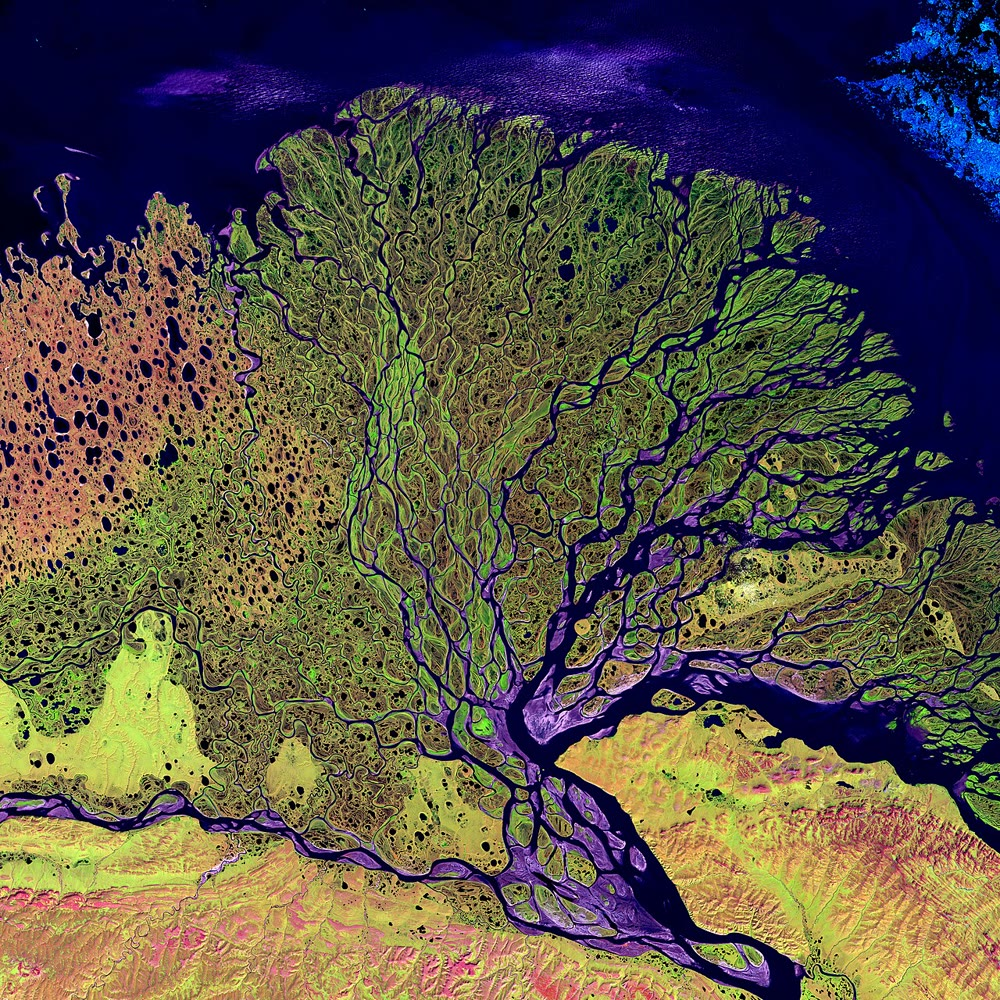
\includegraphics[width=\linewidth]{images/book1/g9-lena-delta.jpg}
\end{minipage}\hfill
\begin{minipage}[c]{0.46\linewidth}\raggedright
{\small De \omterm{def:g5:water-shapes-the-land:delta}{delta} van de \omterm{def:g1:landscapes-around-us:water}{rivier} de Lena, in Siberië, waar ze uitmondt in de
Noordelijke IJszee: een Landsat-beeld in valse kleuren van 27~februari
2000, gemaakt met kortgolvig infrarood, infrarood en rood licht. De vele
geulen van de \omterm{def:g1:landscapes-around-us:water}{rivier} zijn blauw. USGS EROS Data Center, via NASA Visible
Earth (publiek domein, via Wikimedia Commons).}
\end{minipage}
% ledger: commons:lena-landsat
\label{fig:g9:maps-of-the-earth:lena}
\end{omfigure}

\section{Satellietplaatsbepaling}

Een telefoon of een auto kan bijna overal op de Aarde tot op een paar meter
nauwkeurig zeggen waar hij is. Hij ziet de satellieten niet; hij luistert
naar ze.

\begin{definition}[Satellietplaatsbepaling]\label{def:g9:maps-of-the-earth:positioning}
\emph{Satellietplaatsbepaling}\index{satellietplaatsbepaling} is het
bepalen van een positie op de Aarde uit de afstanden tot verschillende
satellieten waarvan de posities bekend zijn. Een ontvanger berekent elke
afstand uit de tijd die een signaal van de satelliet nodig heeft om hem te
bereiken.
\end{definition}

Het Amerikaanse systeem, GPS, houdt minstens 24 werkende satellieten op een
hoogte van ongeveer \qty{20200}{km}. Elk ervan draait twee keer per dag om
de Aarde, in zes banen die rond de planeet zijn verdeeld, zodat vanaf bijna
elk punt op de Aarde minstens vier satellieten zichtbaar zijn. Een signaal
van \qty{20200}{km} ver, dat met de lichtsnelheid reist, komt aan na $20\,200 \div
300\,000 \approx 0.067$~s: de ontvanger meet deze tijd en zet hem om in
een afstand.
% ledger: gps:constellation, const:c (travel time computed in figdata/grade-9/trilateration.py)

Hoe geven afstanden een positie? Stel je het idee voor op een platte \omterm{def:g2:drawing-to-map:map}{kaart}.
Als de ontvanger op \qty{5}{km} van baken~A is, ligt hij ergens op een
cirkel met een straal van \qty{5}{km} rond A. Als hij ook op \qty{10}{km}
van B is, ligt hij op beide cirkels: op een van de twee punten waar ze
elkaar snijden. Een derde afstand, \qty{5}{km} van C, wijst het juiste
punt aan. In de ruimte worden de cirkels bollen, en om dezelfde reden is
er één satelliet meer nodig.

\begin{omfigure}
\begin{minipage}[c]{0.5\linewidth}\centering
\begin{tikzpicture}
\begin{axis}[x=0.42cm, y=0.42cm, xmin=-1, xmax=13, ymin=-1.5, ymax=13,
  ticks=none, axis line style={black!40}]
  \addplot[omSea!70!black, line width=0.6pt] table {figdata/out/grade-9-trilateration-circles.dat};
  \addplot[only marks, mark=triangle*, mark size=2.6pt, point meta=explicit symbolic, nodes near coords,
    nodes near coords style={font=\footnotesize\bfseries, anchor=south west, inner sep=1pt}]
    table[meta=label] {figdata/out/grade-9-trilateration-beacons.dat};
  % labels first (on a white patch), then the points on top of them
  \addplot[only marks, mark=none, point meta=explicit symbolic, nodes near coords,
    nodes near coords style={font=\footnotesize\bfseries, anchor=north east, xshift=-1pt, yshift=-1pt, inner sep=1pt, fill=white, text=red!75!black}, skip coords between index={1}{2}]
    table[meta=label] {figdata/out/grade-9-trilateration-points.dat};
  \addplot[only marks, mark=none, point meta=explicit symbolic, nodes near coords,
    nodes near coords style={font=\footnotesize, anchor=south west, xshift=1pt, yshift=1pt, inner sep=1pt, fill=white}, skip coords between index={0}{1}]
    table[meta=label] {figdata/out/grade-9-trilateration-points.dat};
  \addplot[only marks, mark=*, mark size=2pt, red!75!black, skip coords between index={1}{2}] table {figdata/out/grade-9-trilateration-points.dat};
  \addplot[only marks, mark=o, mark size=2pt, fill=white, skip coords between index={0}{1}] table {figdata/out/grade-9-trilateration-points.dat};
\end{axis}
\end{tikzpicture}
\end{minipage}\hfill
\begin{minipage}[c]{0.46\linewidth}\raggedright
{\small Plaatsbepaling op een platte \omterm{def:g2:drawing-to-map:map}{kaart} (een schets; het raster in
kilometer is niet getekend). De ontvanger R ligt op \qty{5}{km} van A,
\qty{10}{km} van B en \qty{5}{km} van C. De cirkels rond A en B snijden
elkaar in R en in een vals punt F; alleen R ligt ook op de cirkel rond C.}
\end{minipage}
% ledger: (invented region: exercise data, figdata/grade-9/trilateration.py)
\label{fig:g9:maps-of-the-earth:trilateration}
\end{omfigure}

\begin{omfigure}
\begin{minipage}[t]{0.48\linewidth}\centering
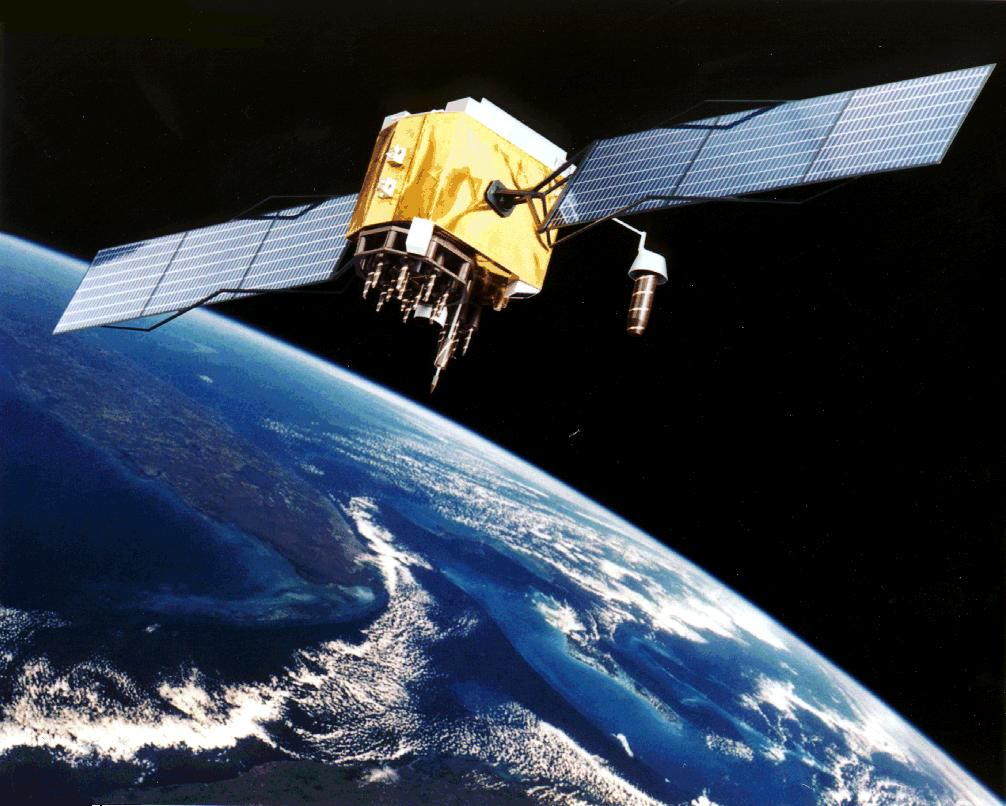
\includegraphics[width=\linewidth]{images/book1/g9-gps-satellite.jpg}

{\small Een GPS-satelliet in zijn baan, zoals een kunstenaar hem zich
voorstelde. NASA (publiek domein, via Wikimedia Commons).}
\end{minipage}\hfill
\begin{minipage}[t]{0.48\linewidth}\centering
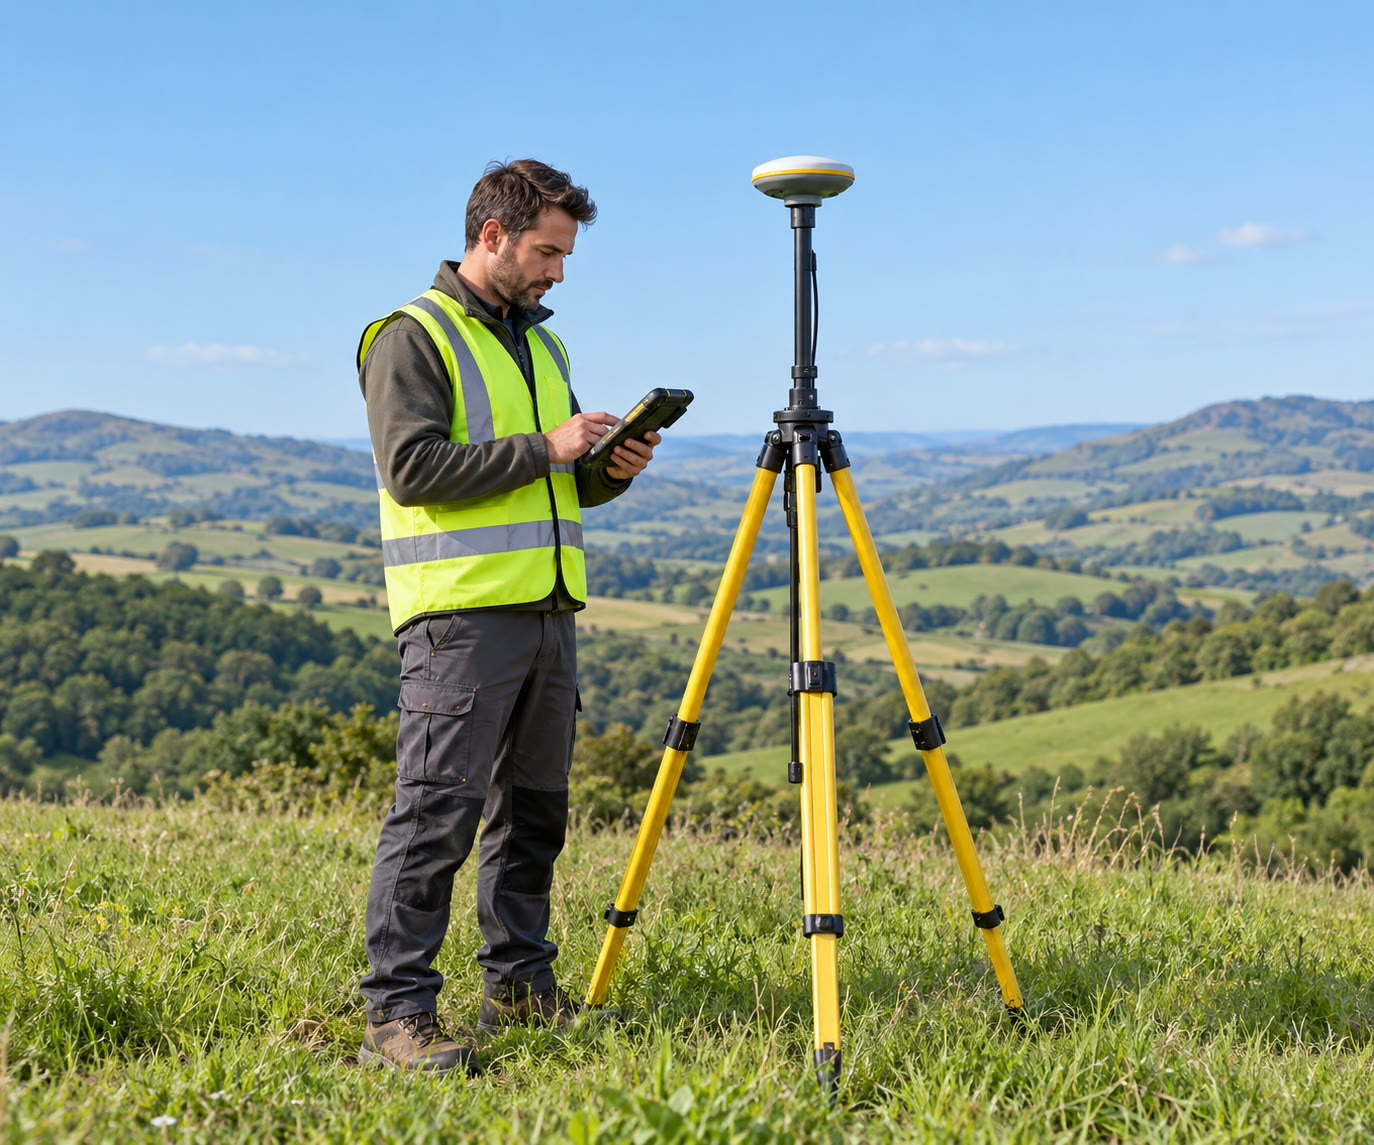
\includegraphics[width=\linewidth]{images/book1/ai/g9-surveyor.jpg}

{\small Een landmeter bepaalt de positie van een punt met een
satellietontvanger op een statief (een illustratie).}
\end{minipage}
% ledger: commons:gps-iif
\label{fig:g9:maps-of-the-earth:gps}
\end{omfigure}

\section{Oefeningen}

\begin{exercise}[$\star$]\label{exo:g9:maps-of-the-earth:1}
Geef het woord bij elke beschrijving. (a) Een regel die elk punt van de
\omterm{def:g3:continents-and-oceans:globe}{globe} naar een punt van een platte \omterm{def:g2:drawing-to-map:map}{kaart} stuurt. (b) Een lijn die punten op
dezelfde hoogte verbindt. (c) Een verhouding zoals $1 : 50\,000$. (d) Het
hoogteverschil tussen twee naburige \omterm{def:g9:maps-of-the-earth:contour}{hoogtelijnen}. (e) De Aarde op afstand
waarnemen, bijvoorbeeld vanuit een satelliet.
\end{exercise}

\begin{exercise}[$\star$]\label{exo:g9:maps-of-the-earth:2}
Zet elke afstand op de \omterm{def:g2:drawing-to-map:map}{kaart} om in een afstand in werkelijkheid, in meter
of kilometer. (a) \qty{4}{cm} op een \omterm{def:g2:drawing-to-map:map}{kaart} van $1 : 25\,000$. (b) \qty{3}{cm}
op een \omterm{def:g2:drawing-to-map:map}{kaart} van $1 : 50\,000$. (c) \qty{2.5}{cm} op een \omterm{def:g2:drawing-to-map:map}{kaart} van
$1 : 1\,000\,000$. (d) Hoeveel centimeter staat op een \omterm{def:g2:drawing-to-map:map}{kaart} van
$1 : 25\,000$ voor \qty{1}{km}?
\end{exercise}

\begin{exercise}[$\star$]\label{exo:g9:maps-of-the-earth:3}
Waar of niet waar? Verbeter de onjuiste zinnen. (a) Een \omterm{def:g3:continents-and-oceans:world-map}{wereldkaart} kan de
hele Aarde tonen zonder iets te vervormen. (b) Op een mercatorkaart lijkt
Groenland groter dan het is. (c) Op een oppervlaktegetrouwe \omterm{def:g2:drawing-to-map:map}{kaart} blijven
de vormen overal behouden. (d) Een \omterm{def:g9:maps-of-the-earth:numerical-scale}{schaalbalk} blijft kloppen als een \omterm{def:g2:drawing-to-map:map}{kaart}
met een kopieerapparaat wordt vergroot.
\end{exercise}

\begin{exercise}[$\star$]\label{exo:g9:maps-of-the-earth:4}
Wat betekent het op een \omterm{def:g9:maps-of-the-earth:topographic-map}{topografische kaart} (a) als de \omterm{def:g9:maps-of-the-earth:contour}{hoogtelijnen} heel
dicht bij elkaar liggen? (b) als ze ver uit elkaar liggen? (c) Wat tonen
gesloten \omterm{def:g9:maps-of-the-earth:contour}{hoogtelijnen} die naar binnen toe hoger worden? (d) Waarom kunnen
twee \omterm{def:g9:maps-of-the-earth:contour}{hoogtelijnen} elkaar nooit kruisen?
\end{exercise}

\begin{exercise}[$\star\star$]\label{exo:g9:maps-of-the-earth:5}
% ledger: data:ne-land (factor 1/cos^2, figdata/grade-9/projections.py)
Op een mercatorkaart worden oppervlakten op een breedte van \ang{60}
4 keer vergroot, en op een breedte van \ang{30} ongeveer 1.33 keer,
vergeleken met de \omterm{def:g3:continents-and-oceans:equator}{evenaar}. (a) Een \omterm{def:g1:landscapes-around-us:water}{meer} van \qty{1000}{km^2} op
\ang{60}\,NB wordt op de \omterm{def:g2:drawing-to-map:map}{kaart} getekend. Welke ware oppervlakte heeft een
\omterm{def:g1:landscapes-around-us:water}{meer} op de \omterm{def:g3:continents-and-oceans:equator}{evenaar} dat even groot is getekend? (b) Twee eilanden met
dezelfde ware oppervlakte liggen op \ang{30} en op \ang{60}. Hoeveel keer
groter lijkt het tweede dan het eerste? (c) Waarom kan de mercatorkaart de
\omterm{def:g3:continents-and-oceans:poles}{polen} nooit tonen?
\end{exercise}

\begin{exercise}[$\star\star$]\label{exo:g9:maps-of-the-earth:6}
% ledger: (invented region: the Varden Hills map of the chapter)
Gebruik de \omterm{def:g9:maps-of-the-earth:topographic-map}{topografische kaart} van de Varden Hills in dit hoofdstuk.
(a) Hoe groot is de \omterm{def:g9:maps-of-the-earth:contour}{equidistantie}? (b) Wat is de hoogte van de top die met
zijn hoogtecijfer is aangegeven, en van de hoofdhoogtelijn er vlak omheen?
(c) De \omterm{def:g1:landscapes-around-us:water}{rivier} stroomt naar het oosten. Ligt de dalbodem hoger in het westen
of in het oosten van de \omterm{def:g2:drawing-to-map:map}{kaart}? (d) Tussen welke \omterm{def:g9:maps-of-the-earth:contour}{hoogtelijnen} liggen de
lijnen langs C--D, ten noorden van de \omterm{def:g1:landscapes-around-us:water}{rivier}, het dichtst bij elkaar? Wat
zegt dat je over de helling daar?
\end{exercise}

\begin{exercise}[$\star\star$]\label{exo:g9:maps-of-the-earth:7}
% ledger: (invented region: profile C--D, figdata/grade-9/varden_topo.py)
Gebruik het profiel C--D in dit hoofdstuk. (a) Op ongeveer welke hoogte
liggen C en D? (b) Wat is de laagste hoogte langs het profiel, en hoe ver
van C ligt dat punt? (c) Hoe lang is de vlakke dalbodem langs C--D? (d) Het
profiel is getekend met een verticale schaal die drie keer is uitgerekt.
Waarom doen kaartenmakers dat vaak?
\end{exercise}

\begin{exercise}[$\star\star$]\label{exo:g9:maps-of-the-earth:8}
Op een \omterm{def:g2:drawing-to-map:map}{kaart} van $1 : 25\,000$ kruist een pad de \omterm{def:g9:maps-of-the-earth:contour}{hoogtelijn} van \qty{200}{m}
en daarna, \qty{2}{cm} verder, de \omterm{def:g9:maps-of-the-earth:contour}{hoogtelijn} van \qty{300}{m}. (a) Hoe groot
is de horizontale afstand tussen de twee punten in werkelijkheid?
(b) Hoeveel stijgt het pad? (c) Hoe groot is de helling, als percentage?
(d) Verderop liggen twee \omterm{def:g9:maps-of-the-earth:contour}{hoogtelijnen} die \qty{100}{m} in hoogte
verschillen \qty{4}{cm} uit elkaar op de \omterm{def:g2:drawing-to-map:map}{kaart}. Is het pad daar steiler of
minder steil? Hoeveel?
\end{exercise}

\begin{exercise}[$\star\star$]\label{exo:g9:maps-of-the-earth:9}
% ledger: usgs:landsat1
Landsat~1 draaide 14 keer per dag om de Aarde en kwam om de 18 dagen over
dezelfde plek. (a) Hoeveel omlopen maakte hij tussen twee passages over
dezelfde plek? (b) Elke omloop duurde 103 minuten. Hoe lang duren
14 omlopen, in uren? (c) Hij was gebouwd om één jaar te werken en werd op
6~januari 1978 uitgeschakeld, vijfenhalf jaar na zijn lancering. Hoeveel
keer zijn geplande levensduur heeft hij gewerkt? (d) Noem één verandering
aan het aardoppervlak die beelden van dezelfde plek, met jaren ertussen
gemaakt, kunnen laten zien.
\end{exercise}

\begin{exercise}[$\star\star$]\label{exo:g9:maps-of-the-earth:10}
% ledger: gps:constellation, const:c
Een GPS-satelliet is ongeveer \qty{20200}{km} ver weg; zijn signaal reist
met ongeveer \qty{300000}{km} per seconde. (a) Hoe lang doet het signaal
erover om aan te komen? Schrijf het antwoord in wetenschappelijke notatie.
(b) Als de klok van een ontvanger $1 \times 10^{-3}$~s verkeerd liep, welke
fout in de afstand zou dat geven? (c) Wat zegt dat je over de klokken die
bij \omterm{def:g9:maps-of-the-earth:positioning}{satellietplaatsbepaling} worden gebruikt?
\end{exercise}

\begin{exercise}[$\star\star\star$]\label{exo:g9:maps-of-the-earth:11}
Op een platte \omterm{def:g2:drawing-to-map:map}{kaart} met een raster in kilometer staat baken A op $(0, 0)$
en baken B op $(10, 0)$. Een ontvanger ligt op \qty{6}{km} van A en
\qty{8}{km} van B. (a) Laat zien dat het punt $(3.6, 4.8)$ op \qty{6}{km}
van A en \qty{8}{km} van B ligt. (b) Geef een ander punt op dezelfde
afstanden van A en B. (c) Een derde baken C staat op $(0, 10)$, en de
ontvanger ligt er ongeveer \qty{6.3}{km} vandaan. Welk van de twee punten
is de ontvanger? (d) Waarom heeft \omterm{def:g9:maps-of-the-earth:positioning}{satellietplaatsbepaling} meerdere
satellieten nodig?
\end{exercise}

\begin{exercise}[$\star\star\star$]\label{exo:g9:maps-of-the-earth:12}
% ledger: data:ne-land (areas, figdata/grade-9/projections.py)
Het Afrikaanse vasteland beslaat ongeveer 29~miljoen~\unit{km^2} en
Groenland ongeveer 2.1~miljoen~\unit{km^2}. (a) Hoeveel keer groter is
Afrika? (b) Op een mercatorkaart worden oppervlakten bij het midden van
Groenland, op ongeveer \ang{72}\,NB, ongeveer 10.5 keer vergroot. Schat de
oppervlakte die Groenland lijkt te hebben. (c) Afrika ligt over de \omterm{def:g3:continents-and-oceans:equator}{evenaar},
waar oppervlakten weinig worden vergroot. Vergelijk je antwoord op (b) met
de oppervlakte van Afrika, en verklaar de wandkaart van het begin van het
hoofdstuk. (d) Welke projectie zou je kiezen om de grootte van de
\omterm{def:g3:continents-and-oceans:continent}{continenten} eerlijk te tonen?
\end{exercise}

\section{Probleem: Een wandelpad door de Varden Hills}

\begin{problem}[{Weekendprobleem --- ontwerpers hebben op de topografische
kaart een wandelpad door de Varden Hills getekend; het eindantwoord is de
lengte van het pad in kilometer en de totale stijging in meter}]
\label{pb:g9:maps-of-the-earth:1}
% ledger: (invented region: the Varden Hills, figdata/grade-9/varden_topo.py, part problem: leg lengths 3.6 / 2.5 / 2.35 cm, spot heights 296 / 143 / 335 / 544 m, 4.2 km, 401 m)
Het wandelpad begint bij een boerderij S, daalt af naar een brug B over de
\omterm{def:g1:landscapes-around-us:water}{rivier}, en klimt dan naar een schuilhut W en verder naar de top T. Elk
traject is recht en gaat alleen omlaag of alleen omhoog. De \omterm{def:g2:drawing-to-map:map}{kaart} heeft een
\omterm{def:g2:drawing-to-map:scale}{schaal} van $1 : 50\,000$; de hoogten van S, B, W en T staan erbij.

\begin{omfigure}
\begin{tikzpicture}
\begin{axis}[x=1.6cm, y=1.6cm, xmin=2, xmax=8, ymin=1.8, ymax=6.2, ticks=none,
  axis line style={black!60}, clip mode=individual]
  \addplot[contour] table {figdata/out/shared-region-contours.dat};
  \addplot[index contour] table {figdata/out/shared-region-index-contours.dat};
  \addplot[river] table {figdata/out/shared-region-river.dat};
  \addplot[only marks, mark=none, point meta=explicit symbolic, nodes near coords,
    nodes near coords align={center}, nodes near coords style={font=\tiny, fill=white, inner sep=0.6pt, text=omContour}]
    table[meta=label] {figdata/out/grade-9-varden_topo-labels.dat};
  \addplot[red!75!black, line width=1pt, dashed] table[x=x_km, y=y_km] {figdata/out/grade-9-varden_topo-path.dat};
  \addplot[only marks, mark=*, mark size=1.6pt, red!75!black, point meta=explicit symbolic, nodes near coords,
    nodes near coords align={right}, nodes near coords style={font=\scriptsize\bfseries, text=black, fill=white, fill opacity=0.8, text opacity=1, inner sep=1pt}]
    table[meta=label] {figdata/out/grade-9-varden_topo-points.dat};
  \coordinate (na) at (axis cs:8.35,5.4);
\end{axis}
\pic at (na) {northarrow};
\end{tikzpicture}

{\small Het wandelpad S--B--W--T op de \omterm{def:g9:maps-of-the-earth:topographic-map}{topografische kaart} van de Varden
Hills (hier verkleind weergegeven; op de oorspronkelijke \omterm{def:g2:drawing-to-map:map}{kaart} van
$1 : 50\,000$ meten de trajecten 3.6, 2.5 en \qty{2.35}{cm}).}
\label{fig:g9:maps-of-the-earth:path}
\end{omfigure}

\noindent\textbf{Deel I --- De route op de kaart.}\par\nopagebreak
\begin{enumerate}[beginpenalty=10000]
  \item Voor hoeveel meter in werkelijkheid staat \qty{1}{cm} van de \omterm{def:g2:drawing-to-map:map}{kaart}
        bij $1 : 50\,000$?
  \item Op de oorspronkelijke \omterm{def:g2:drawing-to-map:map}{kaart} meet het traject S--B \qty{3.6}{cm}. Hoe
        lang is het in werkelijkheid, in kilometer?
  \item De trajecten B--W en W--T meten \qty{2.5}{cm} en \qty{2.35}{cm}.
        Hoe lang zijn ze in werkelijkheid?
  \item In welke algemene richting loopt het pad van B naar T?
\end{enumerate}

\noindent\textbf{Deel II --- De klim.}\par\nopagebreak
\begin{enumerate}[resume, beginpenalty=10000]
  \item Hoe groot is de \omterm{def:g9:maps-of-the-earth:contour}{equidistantie} van de \omterm{def:g2:drawing-to-map:map}{kaart}?
  \item Welk traject gaat omlaag? Hoeveel meter?
  \item Hoeveel meter klimt het pad op B--W, en op W--T?
  \item Wat is de gemiddelde helling van het traject W--T, als percentage?
  \item Waarom hebben de ontwerpers het pad niet in een rechte lijn van S
        naar T getekend?
\end{enumerate}

\noindent\textbf{Deel III --- De wandeling.}\par\nopagebreak
\begin{enumerate}[resume, beginpenalty=10000]
  \item Stel dat een wandelaar op vlak terrein \qty{4}{km} per uur aflegt
        en voor elke \qty{10}{m} klimmen één minuut extra nodig heeft. Hoe
        lang duurt de hele wandeling?
  \item Een andere wandelaarster volgt het pad in omgekeerde richting, van
        T naar S. Hoeveel meter klimt ze?
  \item Wat is de totale lengte van het wandelpad, in kilometer, en de
        totale stijging, in meter?
\end{enumerate}
\end{problem}
